\documentclass[sr]{./../../common/SurferDesc}%%%%%%%%%%%%%%%%%%%%%%%%%%%%%%%%%%%%%%%%%%%%%%%%%%%%%%%%%%%%%%%%%%%%%%%
%
% The document starts here:
%
\begin{document}
\footnotesize
% WeltrekordflŠchen

%%% 1.Tafel

%%%%%%%%%%%%%%%%%%%%%%%%%%%%%


\begin{surferPage}
  \begin{surferTitle}Симетрични седмоугао\end{surferTitle}   \\
    Ова површ која изгледа као звезда је седмог степена. Број његових сингуларитета, $84$, 
	до скоро је сматран максималним бројем реалних сингуларитета за било коју површ седмог степена;
    тек је 2004. Оливер Лабс поправио овај светски рекорд на $99$.
  
  
 Три еластична слоја која се могу видети на овој интерактивној слици, 
    настају због коришћења Чебишевљевих полинома, сличних Чмутовом 
    полиному осмог степена. 
    У ствари, ова површ облика звезде је још једна варијанта Чмутове површи.
    У овом случају, крива у равни $T_d(x)+T_d(y)$ је замењена правилним $7$-углом
    $S_7(x,y)$: 
   \[S_7(x,y) + \lambda \cdot T_d(z) = 0,\]
    за одговарајуће изабрану реалну вредност $\lambda\in\RR$. 
    \vspace*{-0.3em}
    \begin{center}
      \begin{tabular}{c@{\qquad}c}
        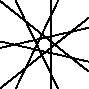
\includegraphics[height=1.5cm]{./../../common/images/labsseptic1.pdf}
        &
        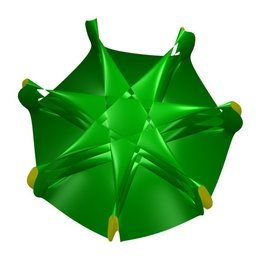
\includegraphics[height=1.5cm]{./../../common/images/septic_7eck_von_oben}
      \end{tabular}
    \end{center}
    \vspace*{-0.3em}   
   Ову варијанту Чмутове конструкције је урадио Дуко ван Стратен. 


  \begin{surferText}
     \end{surferText}
\end{surferPage}



\end{document}
%
% end of the document.
%
%%%%%%%%%%%%%%%%%%%%%%%%%%%%%%%%%%%%%%%%%%%%%%%%%%%%%%%%%%%%%%%%%%%%%%%
